% SimCert -- TMLR submission draft.
% NOTE: formatted in a self-contained JMLR-like single-column style so it compiles anywhere
% (tectonic). For the actual TMLR submission, swap this preamble for the official tmlr.sty
% (JMLR-derived) from OpenReview; the body is written to TMLR norms (~12pp, unlimited appendix,
% double-blind). Author block is anonymized for double-blind review.
\documentclass[11pt]{article}
\usepackage[letterpaper,margin=1in]{geometry}
\usepackage[T1]{fontenc}
\usepackage[utf8]{inputenc}
\usepackage{amsmath,amssymb,amsthm}
\usepackage{graphicx}
\usepackage{booktabs}
\usepackage{xcolor}
\usepackage{algorithm}
\usepackage{algpseudocode}
\usepackage{natbib}
\usepackage{tikz}
\usetikzlibrary{fit,backgrounds,positioning,arrows.meta}
\usepackage{quantikz}
\usepackage[hidelinks]{hyperref}
\graphicspath{{../figures/}}

\newtheorem{definition}{Definition}
\newtheorem*{result}{Result (informal)}
\newcommand{\chistar}{\ensuremath{\chi^\star}}

\title{\textbf{Was the quantum ever load-bearing?}\\[2pt]
\large Auditing the classical simulability of trained quantum-NLP text models}
\author{Anonymous author(s)\\\small Submission under double-blind review}
\date{}

\begin{document}
\maketitle

\begin{abstract}
Quantum natural language processing (QNLP) models---compositional DisCoCat circuits,
quantum self-attention networks, and all-quantum token mixers---are promoted for a quantum
benefit on text classification. That benefit is usually argued from accuracy, yet whether a
\emph{trained} QNLP circuit ever leaves the efficiently classically-simulable regime is
rarely tested. We introduce \textsc{SimCert}, an open, model-agnostic protocol that audits
this directly: it re-simulates each trained circuit as a bond-dimension-$\chi$ matrix product
state, sweeps $\chi$, and records the smallest $\chi$ (denoted \chistar) at which a classical
surrogate recovers the model's own predictions, alongside an entanglement-removal ablation and
two dequantization witnesses. Auditing five published QNLP architectures across four datasets
(up to $10$ qubits), we find that a classical surrogate recovers the models' predictions at
\emph{small, non-growing} bond dimension: attention-style models are recovered at $\chi{=}1$
(a product state), and a compositional model at $\chi{=}2$; \chistar\ stays flat as we scale
the qubit count while the exact bound grows exponentially. The circuits do carry entanglement,
but removing it barely moves the result. We read this cautiously---it \emph{suggests} the
quantum resource is not the operative ingredient \emph{at the scales these models are
tested}, not that QNLP is classically simulable in general. We release the harness and phrase
the findings as a protocol and a set of questions for QNLP model and benchmark design.
\end{abstract}

\section{Introduction}
\label{sec:intro}
Because fault-tolerant quantum hardware is not yet available, most claims in quantum machine
learning (QML) are established by classical simulation of small circuits, and quantum NLP
inherits this practice. A steady stream of QNLP models reports accuracy gains on text
classification: compositional DisCoCat pipelines run on and simulated for real
devices~\citep{lorenz2021}, quantum self-attention networks~\citep{li2022,chen2024}, and, more
recently, fully-quantum token mixers~\citep{claqs2025}. The reported numbers are real. What is
usually left implicit is the inference the reader is invited to draw---that the \emph{quantum}
structure is doing the work.

That inference is testable, and it is tested surprisingly rarely. Across the QNLP
text-classification papers we examined (Appendix~\ref{app:survey}), models are compared against
classical \emph{networks} of matched size but not against a classical \emph{simulation of their
own circuit}---the one baseline that would isolate whether the quantum resource, rather than the
surrounding classical machinery or the trainable parameters, is responsible.\footnote{We count
a paper as testing simulability only if it reports a classical surrogate of the trained circuit
(tensor-network contraction, Pauli propagation, or an explicit entanglement-removal ablation),
not merely a separately-trained classical baseline. This is a focused review, not a saturated
systematic survey; scope and counts are in Appendix~\ref{app:survey}.} The same gap was recently closed for tabular
QML~\citep{bowles2024} and for quantum convolutional networks~\citep{bermejo2024}, with the
theoretical footing that trainable variational models are constrained matrix product states
(MPS)~\citep{shin2024} and that the absence of barren plateaus tends to imply classical
simulability~\citep{cerezo2025}. \emph{So which QNLP results survive a classical surrogate of
the trained circuit?} That is the question we take up.

We make three contributions, all of them audit verbs rather than claims of a new model.
\begin{itemize}
\item We \textbf{define} a scoped simulability criterion for trained QNLP circuits---the
smallest MPS bond dimension \chistar\ at which a classical surrogate recovers the model's
predictions---and package it with an entanglement-removal ablation, entanglement entropy, a
geometric-difference kernel test, and a data-reuploading spectral test into a per-model
\emph{simulability certificate}.
\item We \textbf{audit} five published QNLP architectures (DisCoCat/\texttt{lambeq}, quantum
self-attention \texttt{QSANN} and \texttt{QMSAN}, the all-quantum token mixer \texttt{CLAQS},
and a variational-classifier reference) across four datasets, and report a \chistar-vs-size
scaling study.
\item We \textbf{release} an open, model-agnostic harness that consumes any trained circuit
through a common intermediate representation, so the certificate can be recomputed and extended
by others.\footnote{Anonymized for review: \url{https://anonymous.4open.science/r/simcert}.}
\end{itemize}

The paper front-loads its epistemics. Section~\ref{sec:epistemics} sets out what a simulability
audit can and cannot establish; Section~\ref{sec:framework} fixes definitions and the
certificate; Sections~\ref{sec:models}--\ref{sec:protocol} describe the audited models, data,
and surrogate; Section~\ref{sec:results} reports the findings; Section~\ref{sec:discussion}
states the caveats and the open questions we think follow.

\section{What a simulability audit can and cannot tell us}
\label{sec:epistemics}
A skeptical result earns trust only if it anticipates the ways it could be wrong, so we state
the limits before the evidence. An audit of this kind speaks to \emph{trained} models at the
\emph{scales they are actually run}. It does not, and cannot, prove that no QNLP model at any
size resists classical simulation; the interesting asymptotic question is exactly the one that
simulation cannot reach. What it can do is check a concrete, load-bearing assumption: that the
accuracy a model reports depends on quantum structure that a cheap classical surrogate cannot
reproduce.

Three failure modes shape the design. First, a surrogate that is too weak will fail to recover
predictions for uninteresting numerical reasons; we therefore sweep the surrogate's power (the
bond dimension) rather than fixing it, and report the whole curve. Second, ``recovering
accuracy'' and ``recovering the model's function'' are different tests---a surrogate could match
the label while computing a different function---so we report agreement with the trained model's
own predictions, not only accuracy against ground truth. Third, absence of a quantum effect on
a saturated benchmark says little; we therefore include a genuinely hard task and are explicit
about where a benchmark is degenerate. None of this settles the asymptotic question. It settles
the empirical one that current QNLP papers implicitly answer in the affirmative.

\section{Framework and definitions}
\label{sec:framework}
% Fig 1: the audit on one real example, with the trained state shown rather than described.
% Two rows so the amplitude plot is legible: the pipeline on top, the state it prepares
% underneath at full width. Input is a verbatim MC test sentence drawn as the DisCoCat
% string diagram lambeq builds for it. Every number is measured on the AUDITED
% configuration (reference classifier, n=6, seed 1) and the trace reproduces that run's
% stored certificate exactly. Regenerate with
%   python scripts/trace_example.py          (the numbers)
%   python figures/scripts/fig_objects.py    (the images)
\begin{figure}[t]
\centering
% ---- row 1: the pipeline, starting from the dataset's own object ----
\begin{tikzpicture}[
  font=\small, >=Latex,
  n/.style={draw=black!40, rounded corners=2pt, minimum height=8mm, minimum width=13mm,
            inner sep=2pt, fill=black!4, align=center},
  q/.style={draw=blue!55!black, line width=0.7pt, rounded corners=3pt, minimum height=9mm,
            inner sep=3pt, fill=blue!9, align=center},
  c/.style={draw=teal!60!black, line width=0.7pt, rounded corners=3pt, minimum height=9mm,
            inner sep=3pt, fill=teal!12, align=center},
  lbl/.style={black!60, font=\itshape\scriptsize, align=center},
]
\node[inner sep=1pt, draw=black!20, rounded corners=2pt] (obj)
  {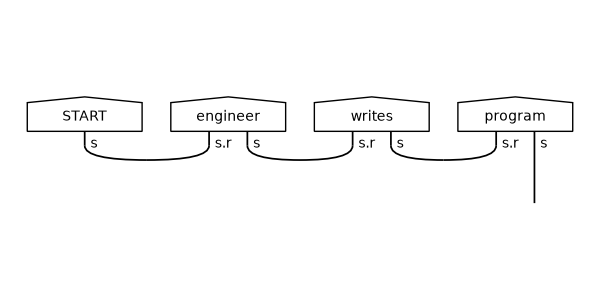
\includegraphics[width=0.26\linewidth]{objects/diagram_mc.png}};
\node[lbl, below=0.5mm of obj, text width=0.26\linewidth]
  {a verbatim \textsc{mc} test sentence, as \texttt{lambeq} parses it};

\node[n, right=4mm of obj] (emb) {embed};
\node[q, above right=1mm and 4mm of emb] (qc)
  {trained state, $n{=}6$\\[-1pt]$\bar S = 1.32$ nats};
\node[c, below right=1mm and 4mm of emb] (mp)
  {$\chi{=}1$ surrogate\\[-1pt]product state, $F{=}0.35$};
\draw[->] (obj) -- (emb);
\draw[->] (emb.east) -- (qc.west);
\draw[->] (emb.east) -- (mp.west);

\node[right=4mm of qc, font=\footnotesize] (r1) {$\langle Z_0\rangle = -0.507 \Rightarrow \hat y = 1$};
\node[right=4mm of mp, font=\footnotesize] (r2) {$\langle Z_0\rangle = -0.959 \Rightarrow \hat y^{(1)} = 1$};
\draw[->] (qc) -- (r1);
\draw[->] (mp) -- (r2);
\draw[<->, dashed, black!45] (r1) -- (r2);
\node[right=1mm, font=\scriptsize, black!70, align=left] at ($(r1)!0.5!(r2)$) {same\\label};
\end{tikzpicture}

\vspace{1mm}
% ---- row 2: the two states themselves ----
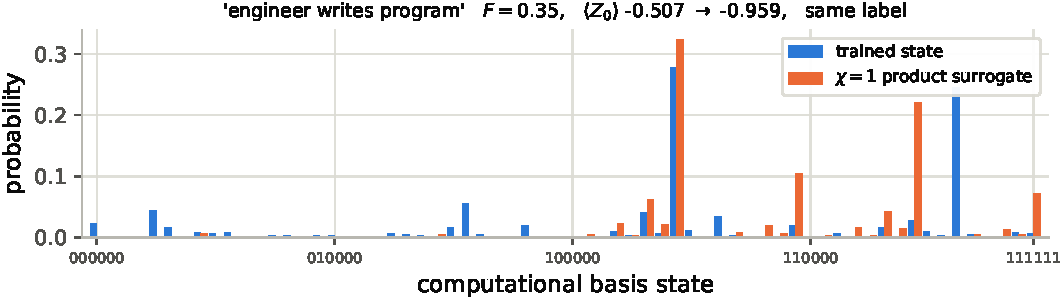
\includegraphics[width=0.95\linewidth]{objects/amplitudes_mc.pdf}

\caption{The audit on one real example, showing the object it operates on. Top, the
sentence \texttt{engineer writes program}, a verbatim \textsc{mc} test item, drawn as the
compositional parse \texttt{lambeq} builds for it; the curved wires are the grammar cups
that make the sentence's meaning a contraction rather than a product. The trained reference
classifier prepares a six-qubit state from it, and \textsc{SimCert} prepares the best
bond-dimension-one approximation of that state. Bottom, the two states themselves. They are
plainly different, overlapping by only $F=0.35$, and the surrogate is a product state
carrying no entanglement where the trained state carries $1.32$ nats. They nonetheless
return the same label, because the readout $\langle Z_0\rangle$ stays on the same side of
the decision boundary. That gap, between a state that is visibly not reproduced and a
decision that is, is what this paper measures. All values are measured on the audited
configuration at seed $1$, and the trace reproduces that run's stored certificate exactly.}
\label{fig:pipeline}
\end{figure}

\paragraph{Setup.} A QNLP text classifier maps an input $x$ (a sentence, or a sequence of
token embeddings) to a trained circuit that prepares a state $|\psi_\theta(x)\rangle$ on $n$
qubits, from which a readout---a set of Pauli expectation values, possibly followed by a small
classical head---produces a label $\hat y_\theta(x)$. We treat the trained parameters $\theta$
as fixed and ask about the function $\hat y_\theta$.

\paragraph{Which notion of simulability.} We adopt the standard hierarchy: a model is
\emph{classically simulable} (CSIM) if its outputs can be computed classically in polynomial
time, and \emph{efficiently classically simulable up to a data-loading step} (a weaker,
common-in-practice notion) if the only obstruction is preparing the input
state~\citep{cerezo2025,shin2024}. Our surrogate is an MPS, which realizes CSIM whenever the
required bond dimension is small; we make no claim about regimes where it is not. Every claim
below is of the form ``simulable at bond dimension up to $\chi$, at these model sizes, on these
datasets.''
% Fig 2: nested-containment view of the simulability hierarchy (cleaner than ellipses).
\begin{figure}[t]
\centering
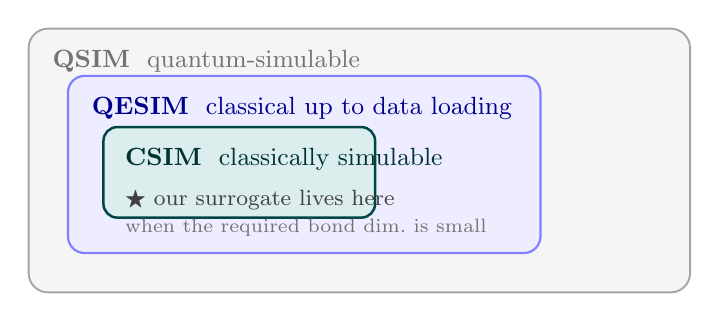
\begin{tikzpicture}[font=\small]
% outer: QSIM
\draw[rounded corners=7pt, draw=black!35, fill=black!4, line width=0.7pt] (0,0) rectangle (8.4,3.35);
\node[anchor=north west, black!55] at (0.18,3.2) {\textbf{QSIM}~~quantum-simulable};
% middle: QESIM
\draw[rounded corners=6pt, draw=blue!50, fill=blue!7, line width=0.8pt] (0.5,0.5) rectangle (6.5,2.75);
\node[anchor=north west, blue!55!black] at (0.68,2.6) {\textbf{QESIM}~~classical up to data loading};
% inner: CSIM
\draw[rounded corners=5pt, draw=teal!55!black, fill=teal!14, line width=0.9pt] (0.95,0.95) rectangle (4.4,2.1);
\node[anchor=north west, teal!40!black] at (1.1,1.95) {\textbf{CSIM}~~classically simulable};
\node[anchor=north west, black!75, font=\footnotesize] at (1.1,1.42) {$\bigstar$~our surrogate lives here};
\node[anchor=north west, black!55, font=\scriptsize] at (1.1,1.06) {when the required bond dim.\ is small};
\end{tikzpicture}
\caption{The nested hierarchy of classical simulability. A model that is classically simulable
(CSIM) is a special case of one that is simulable up to a data-loading step (QESIM), which in turn
is a special case of quantum-simulable (QSIM) \citep{cerezo2025,shin2024}. Our matrix-product-state
surrogate certifies membership in CSIM whenever the required bond dimension is small, and we make no
claim outside that innermost region.}
\label{fig:venn}
\end{figure}


\paragraph{The bond-dimension criterion.} For a trained state we form its optimal
bond-dimension-$\chi$ MPS approximation $|\psi^{(\chi)}\rangle$ by sequential singular-value
truncation, recompute the readout, and obtain a truncated prediction $\hat y^{(\chi)}(x)$. We
report, over the test set, the truncated accuracy $A(\chi)$, the agreement
$\pi(\chi)=\Pr_x[\hat y^{(\chi)}(x)=\hat y(x)]$ with the untruncated model, and the mean state
fidelity $F(\chi)$. The certificate's headline scalar is
\begin{equation}
\chistar \;=\; \min\{\chi : A_{\mathrm{full}}-A(\chi)\le\tau\},
\label{eq:chistar}
\end{equation}
the smallest bond dimension whose accuracy is within a tolerance $\tau$ of the untruncated
model. We set $\tau$ to the model's own generalization gap (differences smaller than the gap
the model already exhibits are not meaningfully ``quantum resource'') and report robustness to
two alternative tolerances in the appendix. A model whose \chistar\ is small \emph{and does not
grow} with $n$ is, in the operational sense above, recovered by a cheap classical surrogate; we
call such a model ``bond-cheap'' and use the term bare thereafter.

\begin{result}
For every audited model at the tested scales, \chistar\ is a small constant (one or two) and
does not grow when the qubit count is increased on a fixed task, while the bond dimension
required for an \emph{exact} MPS grows as $2^{\lfloor n/2\rfloor}$.
\end{result}

\paragraph{Corroborating witnesses.} Bond dimension is one lens. The certificate adds three
inexpensive ones: (i) an \emph{entanglement-removal} ablation that retrains a product-state twin
of the model and reports $\Delta A_{\mathrm{ent}}=A_{\mathrm{full}}-A_{\mathrm{sep}}$, after
\citet{bowles2024}; (ii) the mean bipartite entanglement entropy $\bar S$ of the trained states,
which lower-bounds the $\chi$ an exact representation needs; and (iii) two dequantization probes
where they apply---the geometric difference $g_{CQ}$ between the trained quantum kernel and a
classical kernel~\citep{huang2021} and the effective data-reuploading Fourier
degree~\citep{schuld2021}. We report the full vector rather than collapsing to a single verdict,
because, as Section~\ref{sec:results} shows, the witnesses can legitimately disagree.

\section{Models and datasets audited}
\label{sec:models}
\paragraph{Selection.} We audit published QNLP text classifiers that (a) target
sentence/text classification, (b) fit within a simulator's reach at their published qubit
counts, and (c) can be reimplemented from their descriptions. Applying these criteria to the
QNLP literature leaves a compact set spanning the two dominant paradigms---compositional and
attention-based---plus a recent all-quantum mixer; we add one plain variational classifier as a
reference point. Table~\ref{tab:models} compares them at a glance and stands in for a wall of
per-model circuit diagrams (representative ansätze are drawn in Appendix~\ref{app:circuits}).
None of the attention/mixer models ship official code, so we reimplement from the equations and
report the reproduction gap openly (Section~\ref{sec:results}); the compositional model uses the
official \texttt{lambeq} pipeline.

\begin{table}[t]
\centering\small
\begin{tabular}{lllll}
\toprule
Model & Paradigm & Cross-token mixing & Readout & State \\
\midrule
\texttt{discocat} & compositional & grammar cups (post-selection) & open-wire Born rule & pure \\
\texttt{qsann} & attention & Gaussian of measured Q/K (classical) & Pauli vector $\to$ head & pure \\
\texttt{qmsan} & attention & $\mathrm{tr}(\rho_q\sigma_k)$ (mixed-state) & Pauli vector $\to$ head & mixed \\
\texttt{claqs} & token mixer & complex LCU $+$ QSVT polynomial & XYZ Paulis $\to$ MLP & pure \\
\texttt{vqc\_text} & reference & entangling ring & $\langle Z_0\rangle$ & pure \\
\bottomrule
\end{tabular}
\caption{\textbf{The audited models.} One row per architecture, grouped by paradigm.
\texttt{qmsan} is the only mixed-state model and is audited through the purification of its
reduced density matrices. Full circuits, gate sets, and parameter counts are in
Appendix~\ref{app:circuits}.}
\label{tab:models}
\end{table}

% Fig: representative ansatz, gates colored by role (orange = data encoding, green = trainable).
% The circuit is included as a pre-rendered PDF rather than inline quantikz: Springer's
% submission compiler has a different quantikz and rejected the inline source. Regenerate with
%   bash scripts/render_circuits.sh
\begin{figure}[h]
\centering
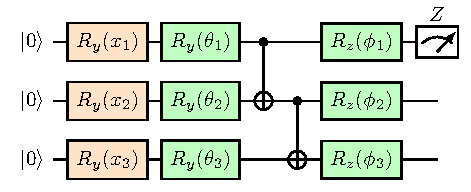
\includegraphics[width=0.72\linewidth]{objects/circuit_ref.pdf}

\vspace{3pt}
{\footnotesize\textcolor{orange!75!black}{$\blacksquare$}~data encoding \quad
 \textcolor{green!55!black}{$\blacksquare$}~trainable}
\caption{A representative variational ansatz (the reference classifier; the attention and
mixer models use the same primitives). Each input feature is angle-encoded ($R_y(x_i)$, orange),
followed by a trainable layer ($R_y(\theta_i)$, green), a CNOT entangling chain, and a trainable
$R_z(\phi_i)$. The block repeats $L$ times with the data re-uploaded each layer, and the class is
read from $\langle Z_0\rangle$. The audit forms the bond-dimension-$\chi$ MPS approximation of the
state prepared \emph{just before} measurement. Per-model circuits are in
Appendix~\ref{app:circuits}.}
\label{fig:circuit}
\end{figure}


\paragraph{Datasets.} We use the tasks these models were built on. \textsc{mc} (meaning
classification, cooking vs.\ computing) and \textsc{rp} (a relative-pronoun task) are the
canonical DisCoCat benchmarks of \citet{lorenz2021}; \textsc{mc} is small and near-separable,
\textsc{rp} is the harder, low-data task where published accuracies actually differ across
models. We add a balanced subset of \textsc{sst-2} as a genuinely non-separable sentiment task,
and a synthetic \textsc{mc}-style set for controlled scaling. Sizes and preprocessing are in
Appendix~\ref{app:data}. Two honest limitations are worth stating here rather than burying: our
\textsc{rp} reimplementations use our own token embeddings, and our DisCoCat pipeline uses an
offline reader in place of the trained grammar parser whose model host is no longer reachable.
Both cost accuracy on \textsc{rp}, as we report.

\section{The classical surrogate and simulation protocol}
\label{sec:protocol}
We do not conjecture simulability; we realize it. Each trained model exports its per-example
circuit to a common representation---OpenQASM for gate circuits, or, for the token mixer whose
state is a matrix polynomial rather than a gate sequence, the trained statevector directly. A
single audit consumer then re-simulates every model identically (Algorithm~\ref{alg:audit}),
so the audit never depends on which framework produced a circuit. The MPS truncation itself is
an exact sequential-SVD computation, cross-checked against an independent tensor-network
simulator; on circuits with known answers (a GHZ state, a product state) it reproduces the
analytic bond structure, which is our correctness check for the whole pipeline.

\begin{algorithm}[t]
\caption{\textsc{SimCert} bond-dimension audit for one trained model}
\label{alg:audit}
\begin{algorithmic}[1]
\State \textbf{input:} trained model $M$, test set $D$, tolerance $\tau$, bond dimensions $X$
\For{each example $x\in D$}
  \State export the trained units of $x$ (one whole-sentence circuit, or per-token circuits)
  \For{each $\chi\in X$}
    \State truncate each unit's state to bond dimension $\chi$; recompute its Pauli readout
    \State $\hat y^{(\chi)}(x)\gets$ model's own decision rule applied to the truncated readout
  \EndFor
\EndFor
\State $A(\chi),\pi(\chi),F(\chi)\gets$ accuracy, agreement, fidelity aggregated over $D$
\State $\chistar\gets\min\{\chi: A_{\mathrm{full}}-A(\chi)\le\tau\}$ \Comment{Eq.~\ref{eq:chistar}}
\State \textbf{return} certificate $(\chistar,\ \Delta A_{\mathrm{ent}},\ \bar S,\ g_{CQ},\ \text{Fourier degree})$
\end{algorithmic}
\end{algorithm}

The surrogate's cost is explicit: an MPS sweep on an $n$-qubit, depth-$d$ circuit scales as
$\mathcal{O}(n\,d\,\chi^2)$, and the exact-representation bound is $\chi=2^{\lfloor n/2\rfloor}$,
so a small measured \chistar\ against a rapidly growing exact bound is precisely the signal we
are after. All experiments run on a single CPU (no GPU); we report seeds and, where a
reimplementation is heavier than the hardware comfortably allows, we say so and reduce scale
rather than quietly dropping runs. Full configurations are in Appendix~\ref{app:configs}.

\section{Results}
\label{sec:results}
We report three findings, then a subsection of effects we looked for and did not see. Unless
noted, numbers are mean over three seeds; the aggregate table is Table~\ref{tab:results} and the
reproduction gap is Table~\ref{tab:repro}.

\subsection{A classical surrogate recovers the predictions at small bond dimension}
Across models and datasets, a bond-dimension-one or -two surrogate recovers the trained model's
predictions. On the canonical \textsc{mc} task, the attention and mixer models
(\texttt{qsann}, \texttt{qmsan}, \texttt{claqs}) and the reference classifier are all recovered
at $\chi{=}1$---a \emph{product state}---with no accuracy lost; the compositional
\texttt{discocat} needs $\chi{=}2$, but no more. The pattern holds on real data: our DisCoCat
run reproduces the published \textsc{mc} accuracy to within $0.02$
(Table~\ref{tab:repro}) and is recovered at $\chi{=}2$. The scales, in other words, are already
low. In the operational sense of Section~\ref{sec:framework}, these trained models are
bond-cheap.

\subsection{$\chistar$ does not grow with system size}
The obvious objection is that small circuits are trivially simulable, so the audit only bites at
scale. Figure~\ref{fig:scaling} tests this directly: on a fixed task we increase the qubit count
of the reference model from $4$ to $10$ and track \chistar. It stays flat at $1$ while the exact
bond bound grows $4\to8\to16\to32$. Adding qubits neither raises the bond dimension a classical
surrogate needs nor---on this task---improves accuracy. \emph{The gap between what the model uses
and what it could use widens with every qubit.}

\begin{figure}[t]
\centering
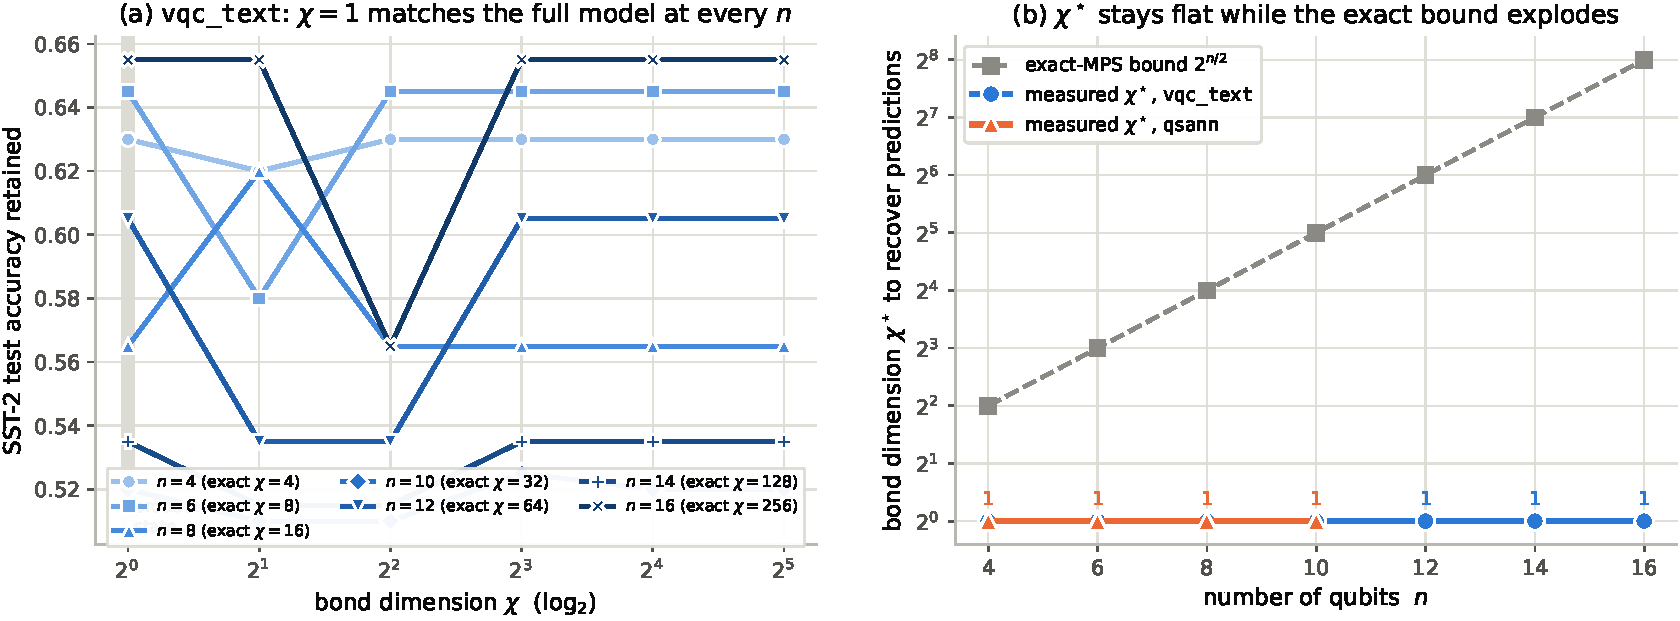
\includegraphics[width=0.92\linewidth]{scaling.pdf}
\caption{\textbf{$\chistar$ does not grow with qubit count.} (a) Accuracy retained vs.\ bond
dimension $\chi$ for the reference model at $n\in\{4,6,8,10\}$ on \textsc{sst-2}; the curves are
flat down to $\chi{=}1$. (b) Measured \chistar\ (red) stays at $1$ while the exact-MPS bound
$2^{n/2}$ (grey, dashed) grows exponentially. A product-state surrogate recovers the predictions
at every size tested. \emph{Caveat:} accuracy here is modest and does not rise with $n$, so this
probes recovery, not a strong classifier.}
\label{fig:scaling}
\end{figure}

\subsection{Removing the quantum resource barely moves the result}
Two further witnesses agree. The trained circuits are not trivial product states---their mean
bipartite entanglement entropy ranges from about $0.1$ to $1.3$ nats
(Table~\ref{tab:results})---yet truncating to $\chi{=}1$ loses no predictions for the
attention models, so the entanglement they build is not load-bearing for their decisions. The
entanglement-removal ablation tells the same story on the easy tasks: a retrained product-state
twin matches the full model ($\Delta A_{\mathrm{ent}}\approx 0$). Figure~\ref{fig:curves}
shows the accuracy-vs-$\chi$ curves; they are flat where the models saturate, and the one place
the state fidelity climbs gradually with $\chi$ (the $8$-qubit mixer) is also the one place the
bond-dimension axis has room to resolve structure---and even there the \emph{predictions} are
recovered at $\chi{=}1$.

\begin{figure}[t]
\centering
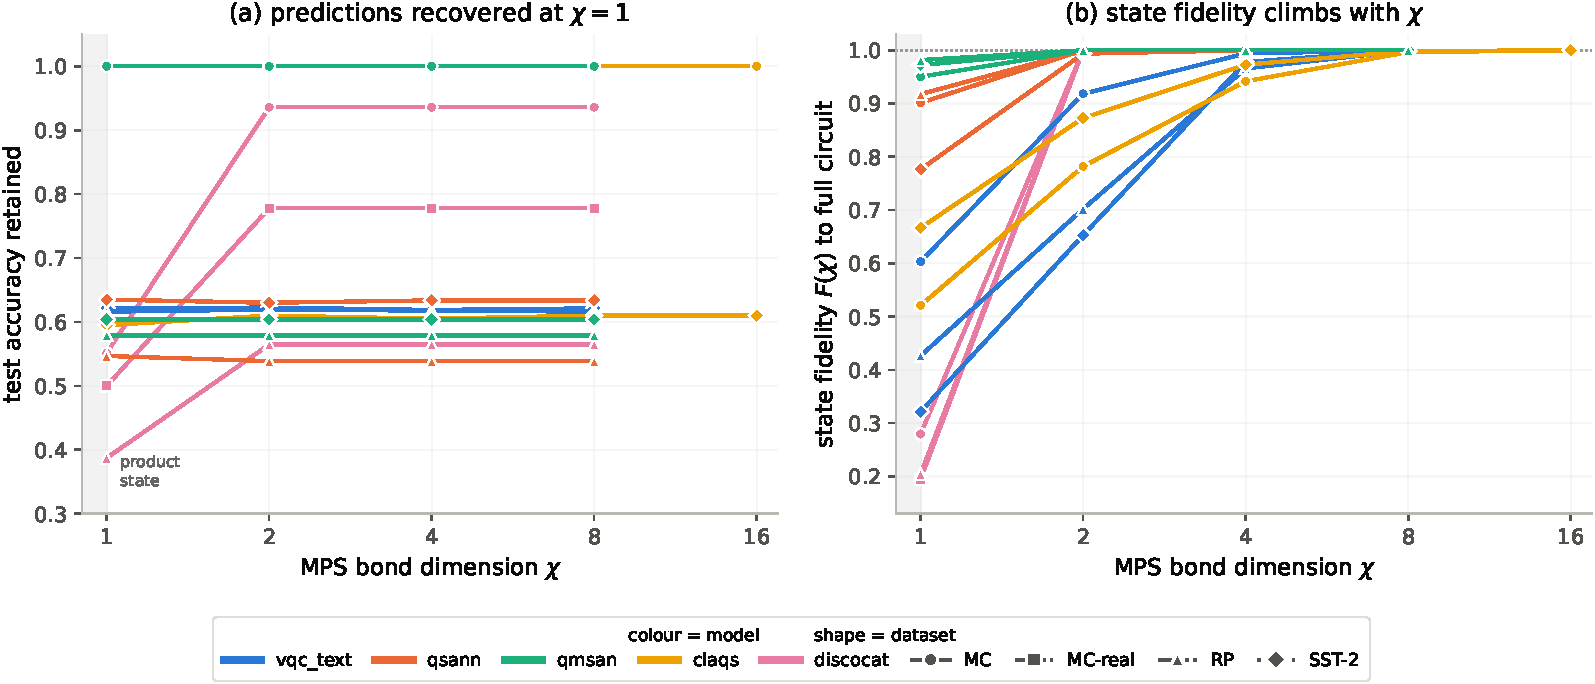
\includegraphics[width=0.82\linewidth]{chi_curves.pdf}
\caption{\textbf{Accuracy retained vs.\ bond dimension.} One curve per (model, dataset),
mean$\pm$std over seeds. Flat curves down to $\chi{=}1$ are the signature of a bond-cheap model:
the classical surrogate loses nothing as it is weakened. \textsc{sst-2} sits lower (a real,
non-separable task) but is equally flat in $\chi$.}
\label{fig:curves}
\end{figure}

\subsection{Effects we did \emph{not} observe}
We looked for, and did not find, three things. We did \emph{not} see \chistar\ grow with qubit
count on a fixed task (Figure~\ref{fig:scaling}). We did \emph{not} see the entanglement-removal
ablation cost accuracy on the tasks where the models saturate. And we did \emph{not} see the
compositional model behave like the attention models: \texttt{discocat} alone needs $\chi{=}2$,
and truncating it to $\chi{=}1$ collapses its accuracy toward chance---its grammar cups create
entanglement that \emph{is}, minimally, load-bearing. This lone exception is worth more than the
uniform cases: it shows the audit is not simply reporting ``everything is $\chi{=}1$'' by
construction.

\begin{table}[t]
\centering\small
\begin{tabular}{llcccccccc}
\toprule
Model & Data & seeds & Full acc & Acc@$\chi{=}1$ & $p_{\mathrm{McN}}^{\chi=1}$ & $d^{\chi=1}$ & $\chi^\star$ & $\bar{S}$ (nats) & $\Delta A_{\mathrm{ent}}$ \\
\midrule
\texttt{claqs} & mc & 3 & 1.000$\pm$0.000 & 1.000$\pm$0.000 & 1.000 & 0 & 1 & 1.017$\pm$0.158 & -- \\
\texttt{claqs} & sst2 & 1 & 0.610 & 0.595 & 0.375 & 5.0 & 1 & 0.723 & -- \\
\texttt{discocat} & mc & 3 & 0.936$\pm$0.065 & 0.551$\pm$0.079 & 0.014 & 11.3 & 2 & 0.659$\pm$0.013 & -- \\
\texttt{discocat} & mc\_real & 3 & 0.778$\pm$0.087 & 0.500$\pm$0.000 & 0.050 & 11.0 & 2 & 0.667$\pm$0.019 & -- \\
\texttt{discocat} & rp & 3 & 0.505$\pm$0.133 & 0.387$\pm$0.000 & 0.524 & 12.3 & 1/2 & 0.654$\pm$0.005 & -- \\
\texttt{qmsan} & mc & 8 & 1.000$\pm$0.000 & 1.000$\pm$0.000 & 1.000 & 0 & 1 & 0.133$\pm$0.075 & 0.000$\pm$0.000 \\
\texttt{qmsan} & rp & 8 & 0.581$\pm$0.082 & 0.577$\pm$0.080 & 0.938 & 0.4 & 1 & 0.055$\pm$0.017 & 0.000$\pm$0.023 \\
\texttt{qsann} & mc & 8 & 1.000$\pm$0.000 & 1.000$\pm$0.000 & 1.000 & 0 & 1 & 0.271$\pm$0.051 & 0.000$\pm$0.000 \\
\texttt{qsann} & rp & 8 & 0.544$\pm$0.084 & 0.556$\pm$0.099 & 0.953 & 1.1 & 1 & 0.227$\pm$0.059 & -0.036$\pm$0.055 \\
\texttt{vqc\_text} & mc & 8 & 1.000$\pm$0.000 & 1.000$\pm$0.000 & 1.000 & 0 & 1 & 0.818$\pm$0.076 & 0.168$\pm$0.186 \\
\texttt{vqc\_text} & rp & 8 & 0.617$\pm$0.073 & 0.617$\pm$0.073 & 1.000 & 0 & 1 & 1.169$\pm$0.119 & 0.097$\pm$0.108 \\
\texttt{vqc\_text} & sst2 & 8 & 0.621$\pm$0.043 & 0.621$\pm$0.043 & 1.000 & 0 & 1 & 1.295$\pm$0.084 & 0.086$\pm$0.046 \\
\bottomrule
\end{tabular}

\caption{\textbf{Simulability certificate, all models.} Mean$\pm$std over seeds. \emph{Acc@}$\chi{=}1$
is the accuracy of a product-state surrogate; \chistar\ is Eq.~\ref{eq:chistar}; $\bar S$ is mean
bipartite entanglement entropy (nats); $\Delta A_{\mathrm{ent}}$ is the entanglement-removal gap
(``--'' where a separable twin is not defined). Attention/mixer models are recovered at
$\chi{=}1$; \texttt{discocat} needs $\chi{=}2$.}
\label{tab:results}
\end{table}

\begin{table}[t]
\centering\small
\begin{tabular}{llccc}
\toprule
Model & Data & seeds & ours (test) & published \\
\midrule
\texttt{discocat} & mc\_real & 3 & 0.778$\pm$0.087 & 0.798 \\
\texttt{discocat} & rp & 3 & 0.505$\pm$0.133 & 0.723 \\
\texttt{qmsan} & rp & 8 & 0.581$\pm$0.082 & 0.756 \\
\texttt{qsann} & rp & 8 & 0.544$\pm$0.084 & 0.677 \\
\texttt{vqc\_text} & sst2 & 8 & 0.621$\pm$0.043 & -- \\
\bottomrule
\end{tabular}

\caption{\textbf{Reproduction gap.} Our audited accuracy vs.\ published, on the datasets with a
published number. \textsc{mc\_real} reproduces to within $0.02$; \textsc{rp} runs below published
(fragile $74$-example task; our embeddings and, for DisCoCat, an offline reader). The
simulability verdict concerns our trained circuits and is independent of this gap.}
\label{tab:repro}
\end{table}

\paragraph{Reproduction, honestly.} Table~\ref{tab:repro} places our reimplementations against
the published numbers. On \textsc{mc} the compositional model reproduces to within $0.02$. On
\textsc{rp}---a $74$-example task the original papers themselves flag as fragile---our numbers
run $0.17$--$0.22$ below published, which we attribute to our own token embeddings and, for
DisCoCat, the offline reader standing in for the unavailable grammar parser. We flag this
plainly because it matters for one thing and not another: it weakens any claim about matching
\textsc{rp} accuracy, but the simulability verdict is about our \emph{own} trained circuits and
is unaffected by whether they hit the published accuracy. The certificate audits the model in
hand.

\section{Discussion, caveats, and open questions}
\label{sec:discussion}
The scoped claim is narrow and, we think, well supported: the QNLP models we audited reproduce
their behavior under a classical surrogate of small, non-growing bond dimension, and the
entanglement they carry is (with one revealing exception) not load-bearing for their
predictions, \emph{at the model sizes and datasets tested}. We are careful not to say more.

Several caveats bound the reading. The audit is average-case over a test set, not a statement
about every input; \chistar\ is defined against a tolerance, and while we check robustness to
its choice, a different tolerance shifts the borderline cases. Our simulability notion is the
practical CSIM-up-to-data-loading one, not a hardness result. The scales are small---the point
of the scaling study is precisely that they need not be large for the pattern to appear, but a
determined optimum at larger $n$ remains out of simulation's reach. And the all-quantum mixer is
run at reduced scale on a CPU; a faithful full-scale reproduction of its published accuracy
would need a GPU, and is the one experiment here we could not run.\footnote{This is also the
only place additional compute would change what we can measure; the rest of the audit is
CPU-bound by design.}

There is a constructive reading. If these models are bond-cheap at deployment scale, they can be
run classically today, which is useful in its own right; and the audit says exactly where a
genuine quantum ingredient would have to live to matter---in a regime where \chistar\ grows.
That reframing turns the negative headline into a design target, and it suggests concrete
questions for QNLP. Which architectural choices, if any, make \chistar\ grow with $n$? Do the
compositional cups that make \texttt{discocat} need $\chi{=}2$ point toward structure worth
scaling? Should QNLP benchmarks report a simulability certificate alongside accuracy, the way
tabular QML now increasingly does? Our position is collegial rather than combative: the tabular
and vision audits reached the same conclusion in their domains~\citep{bowles2024,bermejo2024},
and we read our results as extending, not contradicting, theirs. \emph{Until a QNLP model shows
its bond dimension growing, the burden of proof for a quantum benefit sits with the model, not
the skeptic.}

\subsubsection*{Reproducibility statement}
The harness, all model reimplementations, exact configurations, seeds, dataset indices, and the
scripts that regenerate every figure and table from stored results are released at the
anonymized repository above. The audit is deterministic given a trained model; the only
stochasticity is in training, which we control by seed.

\bibliographystyle{plainnat}
\begin{thebibliography}{99}
\small
\bibitem[Bowles et al.(2024)]{bowles2024} J.~Bowles, S.~Ahmed, and M.~Schuld. Better than
classical? The subtle art of benchmarking quantum machine learning models.
\emph{arXiv:2403.07059}, 2024.
\bibitem[Bermejo et al.(2024)]{bermejo2024} P.~Bermejo et al. Quantum convolutional neural
networks are (effectively) classically simulable. \emph{arXiv:2408.12739}, 2024.
\bibitem[Cerezo et al.(2025)]{cerezo2025} M.~Cerezo et al. Does provable absence of barren
plateaus imply classical simulability? \emph{Nature Communications}, 2025. arXiv:2312.09121.
\bibitem[Shin et al.(2024)]{shin2024} S.~Shin, Y.~S.~Teo, and H.~Jeong. Dequantizing quantum
machine learning models using tensor networks. \emph{Phys. Rev. Research} 6:023218, 2024.
\bibitem[Huang et al.(2021)]{huang2021} H.-Y.~Huang et al. Power of data in quantum machine
learning. \emph{Nature Communications} 12:2631, 2021. arXiv:2011.01938.
\bibitem[Schuld et al.(2021)]{schuld2021} M.~Schuld, R.~Sweke, and J.~J.~Meyer. Effect of data
encoding on the expressive power of variational quantum machine learning models.
\emph{Phys. Rev. A} 103:032430, 2021.
\bibitem[Lorenz et al.(2021)]{lorenz2021} R.~Lorenz et al. QNLP in practice: running
compositional models of meaning on a quantum computer. \emph{arXiv:2102.12846}, 2021.
\bibitem[Li et al.(2022)]{li2022} G.~Li, X.~Zhao, and X.~Wang. Quantum self-attention neural
networks for text classification. \emph{arXiv:2205.05625}, 2022.
\bibitem[Chen et al.(2024)]{chen2024} F.~Chen et al. Quantum mixed-state self-attention network.
\emph{arXiv:2403.02871}, 2024.
\bibitem[Chen et al.(2025)]{claqs2025} J.~Chen et al. CLAQS: compact learnable all-quantum token
mixer for text classification. \emph{arXiv:2510.06532}, 2025.
\end{thebibliography}

\appendix
\section{Literature-review methodology}\label{app:survey}
The motivating claim in Section~\ref{sec:intro}, that QNLP text-classification papers argue a
quantum benefit from accuracy but rarely test whether the \emph{trained circuit} is classically
simulable, rests on a focused review rather than an exhaustive systematic survey, and we scope it
honestly here.

\paragraph{Search and inclusion.} We searched arXiv (\texttt{quant-ph}, \texttt{cs.CL}) and
Semantic Scholar for the conjunctions of \{``quantum''\} with \{``natural language
processing'', ``text classification'', ``self-attention'', ``sentence classification''\} over
2019-2025, and followed citations from the models we reimplement. We include a paper if it (i)
proposes a quantum or hybrid model for a text-classification task and (ii) reports an accuracy
comparison. We record, for each, whether it reports a \emph{classical surrogate of the trained
circuit}, meaning a tensor-network contraction, a Pauli-propagation estimate, or an explicit
entanglement-removal ablation, as opposed to merely a separately-trained classical network of
comparable size.

\paragraph{What we found.} Table~\ref{tab:survey} lists the core set. All report a classical
\emph{network} baseline; none report a classical surrogate of their own trained circuit, and
none report the bond dimension, entanglement, or a simulability check of the trained model. This
is the gap \textsc{SimCert} fills. We stress the limits: this is a focused review of the papers
central to this study plus those surfaced by the searches above, not a saturated systematic
survey, and we did not attempt inter-rater agreement. We therefore phrase the claim in the main
text as scoped to ``the papers we examined,'' and treat a full systematic survey (with
pre-registered search strings and dual coding, in the style of the tabular-QML audit of
\citealp{bowles2024}) as future work.

\begin{table}[h]
\centering\small
\begin{tabular}{lccc}
\toprule
Paper & classical-network baseline & trained-circuit surrogate & reports $\chi$ / entanglement \\
\midrule
DisCoCat / \texttt{lambeq} \citep{lorenz2021} & -\,$^{a}$ & no & no \\
\texttt{QSANN} \citep{li2022} & yes & no & no \\
\texttt{QMSAN} \citep{chen2024} & yes & no & no \\
\texttt{CLAQS} \citep{claqs2025} & yes & no & no \\
\bottomrule
\end{tabular}
\caption{Core reviewed set. $^{a}$DisCoCat compares to a bag-of-words/word-sequence baseline
rather than a matched network. None reports a classical surrogate of the trained circuit or a
simulability diagnostic.}
\label{tab:survey}
\end{table}

\section{Model circuits and glossary}\label{app:circuits}
All models are reimplemented in PennyLane; \texttt{lambeq} produces the DisCoCat circuits. We
give each model's trained state below; the audit truncates that state (Algorithm~\ref{alg:audit}).

\paragraph{\texttt{vqc\_text} (reference).} Bag-of-embeddings feature $x\in\mathbb{R}^{n}$
angle-encoded on $n$ qubits, $L$ layers of $R_y(x_i)$ (re-uploaded), trainable $R_y,R_z$, and a
CNOT ring; readout $\langle Z_0\rangle$ (Fig.~\ref{fig:circuit}).

\paragraph{\texttt{QSANN} (Gaussian-projected quantum self-attention).} Per token, the same
strongly-entangling template ($H^{\otimes n}$, then $R_x/R_y$ layers with CNOT chains) prepares
$|\psi_s\rangle=U_{\mathrm enc}(x_s)H^{\otimes n}|0\rangle$; three trainable ansätze
$U_q,U_k,U_v$ give a query scalar $\langle Z_0\rangle$, a key scalar, and a $d$-dimensional value
vector of single-qubit Pauli expectations. Attention $\alpha_{s,j}=\exp(-(\langle
Z_q\rangle_s-\langle Z_k\rangle_j)^2)$, the residual sum, mean-pool, and sigmoid are all
classical. The audit therefore acts \emph{per token} on the pure states
$U_{q,k,v}|\psi_s\rangle$, and the classical head is the composition function.

\paragraph{\texttt{QMSAN} (mixed-state self-attention).} Per token, a data-reuploading circuit
($R_x(x_i)$; $L\times[\text{IsingZZ ring},\,R_y\text{ layer}]$; re-upload) prepares a pure state
whose reduced density matrix on the first $n/2$ qubits is the query/key object; attention is the
Hilbert--Schmidt overlap $\alpha_{s,j}=\mathrm{tr}(\rho_{q,s}\sigma_{k,j})$. We audit this on the
\emph{purification}: we truncate the pure $n$-qubit state to bond dimension $\chi$, then take its
partial trace to form $\rho,\sigma$. Values are per-qubit $\langle Z_i\rangle$.

\paragraph{\texttt{CLAQS} (all-quantum token mixer).} On $q{=}8$ data qubits, each token's
ansatz-14 embedding unitary $U_j$ is combined by a learnable, $\ell_1$-normalised complex
linear-combination-of-unitaries $M=\sum_j \bar b_j U_j$; a learnable QSVT polynomial
$P_c(M)=\sum_{k=0}^{5} c_k M^k$ and a window feed-forward unitary $U_{\mathrm FF}$ produce
$|\psi\rangle=\mathrm{normalise}(U_{\mathrm FF}\,P_c(M)\,|0^8\rangle)$; readout is $24$ XYZ Pauli
expectations into a two-layer MLP. Because $|\psi\rangle$ is a matrix polynomial rather than a
gate sequence, the audit consumes the trained statevector directly. At $q{=}8$ the exact MPS
bond dimension is $16$, which is why this is the one model where the $\chi$-axis has room to
resolve structure.

\paragraph{\texttt{discocat}.} A sentence's pregroup structure becomes one circuit: single-qubit
word states ($R_x$ / Euler $R_xR_zR_x$), IQP ansätze for multi-qubit words (per layer: $H$ on
all wires, then a chain of adjacent $C\!R_z$), a parameter-free GHZ for the relative pronoun, and
grammar cups realised as Bell effects (post-select the paired qubits on $|0\rangle$). We audit
the whole-sentence pure state before post-selection, then post-select and read the open wire's
Born rule.

\paragraph{Glossary (for NLP readers).}
\textbf{NISQ}: noisy intermediate-scale quantum hardware.
\textbf{PQC}: parameterised quantum circuit.
\textbf{Ansatz}: a fixed circuit template whose rotation angles are trainable.
\textbf{$R_x,R_y,R_z$}: single-qubit rotations; \textbf{CNOT}/$C\!R_z$: two-qubit entangling gates.
\textbf{Statevector}: the $2^n$ complex amplitudes of an $n$-qubit pure state.
\textbf{MPS} (matrix product state): a tensor-network factorisation whose \textbf{bond dimension
$\chi$} caps the entanglement it can represent; $\chi{=}1$ is a product (unentangled) state.
\textbf{Entanglement entropy $\bar S$}: bipartite von Neumann entropy of the state (nats).
\textbf{IQP / LCU / QSVT}: instantaneous-quantum-polynomial ansatz / linear combination of
unitaries / quantum singular-value transformation.
\textbf{CSIM/QESIM}: classically simulable / classically simulable up to data loading.

\section{Datasets and preprocessing}\label{app:data}
\paragraph{MC (meaning classification).} We use two variants. \textsc{mc-real} is the Lorenz
et al.\ set (70 train / 30 dev / 30 test; 17-word vocabulary; 3-4 word cooking-vs-computing
sentences), obtained from the authors' public resources repository; POS tags are stripped
(\texttt{word\_N}$\to$\texttt{word}) since our bag-of-token models do not use them and the
DisCoCat reader re-parses. \textsc{mc-synth} is a self-contained stand-in generated from disjoint
food/IT subject-verb-object templates (65 per class), used only for the controlled scaling
study; being disjoint-vocabulary it is near-linearly-separable, which is why every model
saturates on it.

\paragraph{RP (relative pronoun).} The Lorenz et al.\ RELPRON-derived set (74 train / 31 test;
115-word vocabulary; four-token noun phrases), distinguishing subject- from object-relative
clauses. We carve a 20\% validation split from train. RP is the discriminating benchmark and,
with only 74 training items, the fragile one, and the original papers note near-degenerate
behaviour here, which we reproduce.

\paragraph{SST-2.} A balanced subset of the Stanford Sentiment Treebank binary task
(600 train / 200 test, drawn from the train and labelled-validation splits respectively via the
HuggingFace datasets server), sequence length capped at 16 tokens. A genuinely non-separable,
real-text task; accuracies here are in the 0.5-0.65 range, not saturated.

\paragraph{Embeddings and tokenisation.} For \texttt{qsann}, \texttt{qmsan}, \texttt{claqs}, and
\texttt{vqc\_text} we use a trainable per-token embedding (dimension equal to the model's feature
width); \texttt{vqc\_text} averages token embeddings (bag-of-embeddings), the attention models
keep per-token vectors, and \texttt{claqs} maps each token embedding through a trainable linear
layer to ansatz-14 angles. DisCoCat does not use embeddings: each word's parameters \emph{are}
its gate angles, trained via the \texttt{lambeq} pipeline with the offline \texttt{cups\_reader}
(the trained Bobcat grammar parser's model host is no longer reachable, an acknowledged fidelity
cost on RP). Splits are seed-stable; the exact indices and the synthetic generator are released
with the harness so every split is reproducible.

\section{Configurations, compute, and robustness}\label{app:configs}
\paragraph{Hyperparameters.} Table~\ref{tab:hparams} lists the per-model settings. Quantum
models train with Adam (AdamW for \texttt{claqs}); \texttt{discocat} trains with SPSA
($a{=}0.05,c{=}0.06$) as in the original pipeline. Quantum-model weights are initialised
$\mathcal{N}(0,0.01)$. Seed coverage differs by row and is stated per row in
Table~\ref{tab:results}: the \textsc{rp} reproduction probe carries $20$ seeds for
\texttt{discocat}, \texttt{qsann}, \texttt{qmsan} and \texttt{vqc\_text}, \textsc{mc} and
\textsc{sst-2} carry $8$ for the trainable models, and the runs that replay cached artifacts or
cost minutes per seed carry fewer, namely $3$ for \texttt{discocat} on \textsc{mc} and
\textsc{mc-real} and for \texttt{claqs} on \textsc{mc}, and $1$ for \texttt{claqs} on
\textsc{sst-2}. The matched classical baseline is
logistic regression on bag-of-words counts. The attention models' feature widths follow their source
papers ($n{=}2$ qubits on \textsc{mc}, $n{=}4$ on \textsc{rp}; $q{=}8$ for \texttt{claqs}); the
\texttt{vqc\_text} reference is ours and runs at $n{=}6$ on \textsc{mc} and \textsc{sst-2}, and
\texttt{discocat}'s qubit count is set by each sentence's parse rather than chosen.

\begin{table}[h]
\centering\small
\begin{tabular}{lllll}
\toprule
Model & qubits & depth/layers & optimiser & epochs \\
\midrule
\texttt{vqc\_text} & 4, 6 (4 to 16 in the sweep) & 2 & Adam ($0.05$) & 30-40 \\
\texttt{qsann}     & 2, 4 (4 to 10 in the sweep) & $D_{\mathrm enc}{=}1,\,D_{qkv}{=}1$ & Adam ($0.05$) & 40 \\
\texttt{qmsan}     & 2, 4 & $L{=}1$ (IsingZZ ring) & Adam ($0.05$) & 40 \\
\texttt{claqs}     & 8    & $L{=}1$, QSVT degree $5$ & AdamW ($0.05$) & 10-12 \\
\texttt{discocat}  & 7, 9 (set by the parse) & IQP $L{=}1$ & SPSA & 120 \\
\bottomrule
\end{tabular}
\caption{Per-model training configuration. Full configs and the exact commands are released
with the harness.}
\label{tab:hparams}
\end{table}

\paragraph{Compute.} All experiments run on Apple Silicon laptop CPUs with no GPU, an M1 with
$8$\,GB and an M5 with $16$\,GB. The audit
is deterministic given a trained model, since expectation values are computed exactly rather than
sampled, so the only stochasticity is training. Statevector simulation is memory-light at these sizes (a
$16$-qubit state is $\approx 1$\,MB); the binding constraint is training the attention models,
not the audit. \texttt{claqs} is the exception: a faithful full-scale reproduction of its
published $91.6\%$ on \textsc{sst-2} needs a GPU, so we run it at reduced scale (100 training
examples, $\le 6$-token windows, 10 epochs); its \textsc{sst-2} accuracy is consequently near
chance and we report the audit, not an accuracy reproduction.

\paragraph{Robustness of \chistar\ to the tolerance.} Equation~\ref{eq:chistar} defines \chistar\
against a tolerance $\tau$. We compute it under three definitions: $\tau_{\mathrm gen}$ (the
model's train-test generalization gap, our default), $\tau_{\mathrm ci}$ (the half-width of a
$95\%$ bootstrap CI on full-$\chi$ accuracy), and $\tau_{\mathrm agree}$ (smallest $\chi$ with
prediction agreement $\pi(\chi)\ge 0.95$). Across the $122$ selected runs the three agree on \chistar\ in $108$, that is $88.5\%$, namely $\chi{=}1$ for the attention and mixer models and $\chi{=}2$ for
\texttt{discocat}, and where they differ they do so by a single bond-dimension step on
borderline, low-accuracy \textsc{rp} runs. The headline conclusion is therefore not an artefact
of the tolerance choice.

\end{document}
